\documentclass{article}

\title{A fast and accurate zebra finch syllable detector}
\author{Ben Pearre, L. Nathan Perkins, Jeffrey E. Markowitz, Timothy J. Gardner}

\usepackage{amsmath, amsthm, amssymb, wasysym, graphicx}
\usepackage[small, hang, bf]{caption}
\usepackage{natbib}
\renewcommand\cite{\citep}
\newcommand\citepossessive[1]{\citeauthor{#1}'s \citeyearpar{#1}}
\newcommand\eq[1]{Equation~\ref{#1}}
\newcommand\fig[1]{Figure~\ref{#1}}


\setlength{\marginparwidth}{35mm}
\let\oldmarginpar\marginpar
\renewcommand\marginpar[1]{\-\oldmarginpar[\raggedleft\footnotesize #1]
  {\raggedright\footnotesize #1}}


\newcommand\argmin{\mathop{\mbox{{\rm argmin}}}\limits}
\newcommand{\noprint}[1]{}


\hyphenation{cross-valid-ation}

\begin{document}
\maketitle

\begin{abstract}
  We present an accurate, versatile, and fast syllable detector that
  can control hardware at precisely timed moments during zebra finch
  song. Most moments during song can be isolated and detected with
  $>95$\% accuracy, easier syllables exceed 99.5\% detection, and
  false positive rates can be $<1\%$\marginpar{How to explain how to
    quantify this in the abstract?}. The detector can run on a stock
  Mac Mini with a triggering delay around 1 millisecond and trigger
  jitter with $\sigma\approx 3$ milliseconds.
\end{abstract}

\section{Introduction}

The adult zebra finch sings a song made up of 2-6 syllables, with
longer songs taking on the order of a second. The song may be repeated
hundreds of times per day, and is almost identical each time. This
consistency presents a unique opportunity to study the neural basis of
learning, audition, and control: we do not know of another model in
which \marginpar{Quantify? Remove vacuous handwaving? Figure?} neural
activity may be so easily correlated with motor output.

In order to take advantage of this consistency, it is useful to be
able to detect selected moments during song, in order to align data or
trigger\marginpar{Examples?} other systems.  To the best of our
knowledge, current systems require expensive hardware, extensive
hand-tuning, and careful choice of an easy syllable.

We developed a standalone detector based on the song
spectrogram. Given a set of aligned songs, our software computes
spectrograms and trains a neural network to output a TTL pulse at the
chosen moment. The approach consists of three steps:

\begin{enumerate}
\item Align songs. This is outside the scope of this paper, but we
  provide a pointer to our song alignment software in
  Section~\ref{sec:resources}.
\item Choose one or more desired trigger
  syllables\marginpar{Terminology: ``syllable'' is a unit, but this
    detector triggers on ``song moments'' or something?}, and train a
  neural network to recognise them. This is carried out offline using
  any recent version of Matlab, and we recommend a computer with at
  least 32GB of RAM.
\item Once trained, the Matlab output file is used by a realtime
  detection program written in Swift, which uses the Mac's stereo
  audio jack and the Core Audio interface. Detection of the target
  syllables is indicated by a TTL pulse. Hardware requirements for this
  system are minimal: we use the current (2015) Mac Mini, which is
  overkill.
\end{enumerate}

We present the method in Section~\ref{sec:method}.
Section~\ref{sec:quantify} describes how we define and test
performance.  Section~\ref{sec:results} presents our measurements.
Section~\ref{sec:case} gives an example usage case of the detector. We
conclude in Section~\ref{sec:conclusion}, and point to software
resources in Appendix~\ref{sec:resources}.


\section{Method}
\label{sec:method}

\subsection{Learning a detector}

We begin with a few hundred time-aligned recordings of a given bird's
song.

One or more moments during the song must be chosen.  Our interface
presents the time-aligned spectrogram and requires manual input of the
target times. The user may next tune the region in frequency and time
used for syllable identification. Then we assemble the training set
from the song data, train the network, compute optimal output unit
thresholds, and save the
network file and an audio test file.


\subsubsection{Recognition region}

The neural network uses several concurrent timesteps from the song
spectrogram.  The range of frequencies $F$ and length of the history
$T$ of this recognition region should be chosen in order to contain
unique features of the target syllable and surrounding areas. This
process could perhaps be automated, but we have not done so, as
hand-choosing is neither difficult nor particularly error-prone.

\subsubsection{Song micro-realignment}

As conditions change, and especially during undirected song, syllable
length and relative timing may vary slightly, which introduces
variations in the precise timing of each syllable. The alignment
software we use ensures that songs are aligned at the point midway
through the song, but if the target syllable is not at that point, it
is helpful to re-align the songs at the point of interest.  This may
be accomplished by looking for peaks in the correlation of the
time-domain signal with the song whose spectrogram is closest to
average over the training set.\marginpar{I hope that's the right thing
  to do. Seems to work, anyway\dots}

\subsubsection{Normalisation}

To accommodate differences in amplitude, due to changes in the relative position between the microphone and bird or due to other \marginpar{What data is each norm computed over? Why does this do more than just the second step?}
minor variations in recording, normalisation ensures that the 
detector is sensitive only to the relative spectral content. We found 
that a two-step normalisation works. The spectrogram in the time and 
frequency windows, in decibels, is normalised to have mean zero and 
unit standard deviation. This eliminates relative differences in song
amplitude due to microphone position or line levels. Next, each 
time-frequency bin is normalised based on the training set, such that
that bin has mean zero and unit variance. This scales each 
time-frequency bin based on the amplitudes seen in the training set.
These two normalisation steps provide a set of inputs that were more
robust to outliers and less likely to produce false positives during 
silence when evaluated against other normalisation schemes, such as 
linear or L2 normalisation. \marginpar{Would it be worth putting in
data to this effect?}

\subsubsection{Building the training set}

The neural network's training set is created in the typical fashion:
the rectangular $F\times T$ recognition region in the spectrogram is
simply reshaped into a vector of length $FT$. The requency range is constant,\marginpar{awkward phrasing} and every possible value for $T$ is converted into a training input vector.

With inputs well outside the space on which a neural network has been
trained, its outputs will be essentially random. In order to reduce
the false positive rate it is necessary to provide negative training
examples that include silence, cage noise, non-song vocalisations, and
perhaps songs from other birds. We have found that training with
roughly a 8:1 ratio of non-song to song yields excellent results,
although this will depend on the makeup of the non-song data.

Training targets are, roughly, 1 if the input vector comes from the
target time, 0 otherwise, for each target syllable. Since the song
realignment may not be perfect, due to sample aliasing, and because the song spectrogram appears not to vary faster than the frame rate we chose, a strict binary target may ask the network to learn that practically identical samples should have opposite targets. Thus it is preferable to spread the output
vector in time, such that at the target moment it is 1,
and at neighbouring moments it is nonzero. We found that a Gaussian
smoothing kernel around the target time with $\sigma\simeq 3$ms serves
well.

\subsubsection{Training the network}

The network is trained using Matlab's neural network toolbox. We tried
a variety of feedforward neural network geometries, from simple
1-layer perceptrons to more complicated forms and many hidden
nodes. Perhaps surprisingly, even the former yields excellent results
on many syllables, but a 2-layer perceptron with a very small hidden
layer---just 1 or 2 more units than the number of target
syllables---was a good compromise between accuracy and training
speed. Various other neural network geometries could be tried, as well
as any other classifier that executes quickly.  For more variable
songs, deep structure-preserving networks may be more appropriate, but
they are slow to train and unnecessary for zebra finch song.

Matlab's neural network toolbox defaults to Levenburg-Marquardt
training. This is a fast algorithm, but is memory-intensive, \marginpar{Didn't you guys try reducing input size with an autoencoder? Wasn't that effective?} so
multiple output syllables or high FFT frame rates require a large
amout of RAM and increase training time to hours. Other training
algorithms that use less RAM are much slower, and by default they will
often terminate before converging due to their performance gradient
going to 0.

\subsubsection{Computing optimal output thresholds}
\label{sec:optimalthresholds}
When the network is trained, outputs of the classifier for any input
are now available, and will be in the \marginpar{Or is it (-1, 1)?}
interval (0, 1). We must choose a threshold above which the output is
considered a positive detection. Finding the optimal threshold
requires two choices. The first is the relative cost of false
negatives to false positives, $C$. The second is the acceptable time
interval: if the true event occurs at time $t$, and the detector
triggers at any time $t\pm\Delta t$, then it is considered a correct
detection. Then the optimal detection threshold $\tau$ is the one that
minimises $\mbox{[false positives]} +C\cdot\mbox{[false negatives]}$
over the training set, using the definitions of false positives and
negatives given in Section~\ref{sec:accuracy}. Since large
portions of the cost function are flat, random-restart hillclimbing
would be effective, but a brute-force search requires fractions of a
second. For the results presented here, we have used $C=1$ and $\Delta
t=20$ms.\marginpar{I chose this large value for $\Delta t$ before I
  did target syllable realignment, and it could probably be much
  reduced now. Does this number make our results look bad? Should I
  explain it, change it and rerun, etc?}

\subsubsection{Our parameter choices}

We use a size-256 FFT, a Hamming window, and a spectrum sampled every
2 milliseconds.\marginpar{Check with Nathan and Jeff on what they've
  used.}  We usually define the network's input space to be 20-80ms
long, and to span frequencies from about 1.5-7kHz, which contains the
fundamentals and several overtones of most zebra finch vocalisations.

\marginpar{The parameters used varied form iteration to iteration.
Towards the end, we were using either 128 or 256 size FFT with 
no overlap (or even a gap between the FFTs). Jeff may be able to 
give a better sense of what worked best for him. - NP}

We found these parameters to work well across a variety of target
syllables, but various parameter sets yield results similar to those
presented here.  Some of the parameters trade off detection accuracy
or detection timing vs.~training time. For example, detection latency
and jitter cannot be less than the FFT frame rate, but reducing the
frame rate increases the size of the training set and thus the
training resources required (and also increases the computational
burden on the realtime detector, but that seems low to begin
with).

\subsection{Realtime detection}

In order to implement the trained syllable detector in an 
experimental context, we implemented a realtime detector that runs
off consumer hardware. Using Core Audio frameworks available on 
Mac OS X computers and a low-level language (Swift), we were able
to implement the syllable detector in a way that ensures near-
realtime detection and minimal jitter in detection time.

The Core Audio frameworks provide an adjustable buffer size for 
reading from and writing to audio hardware. Tuning this buffer size
provides a tradeoff between the jitter in the detection and the 
processor usage needed to run the detector. We settled on a buffer 
size of 32 samples (0.7ms at 44.1kHz), as this created minimal system
load while achieving detection within the desired lag and jitter.

Audio samples from the microphone are appended to a circular buffer. 
When there are sufficient samples in the buffer, the spectrogram is
calculated by applying the Hamming window, performing an FFT and 
extracting the power. All vector operations are performed using the
Accelerate framework (vDSP and vecLib), which use modern vector-oriented processor instructions to perform calculations. Outputs
of the spectrogram, from the target frequency band, are appended 
to a second circular buffer. When there is sufficient data in the
second circular buffer, the data is sent to a static implementation
of the neural network previously trained, again implemented using
the Accelerate framework to optimize normalization, matrix 
multiplication and all transfer functions.

The output of the neural network is written to the audio output 
buffer (again, in 32 sample or 0.7ms chunks) to create a trigger 
pulse, which can be used to trigger experimental feedback.

The above code can be run on multiple channels of audio on 
consumer hardware (such as a 2015 Mac Mini) with little impact
on CPU usage ($<15\%$). Depending on the experimental needs, latency
can be further decreased (at the expense of processor usage) by
adjusting the audio buffer sizes.

\section{Quantification}
\label{sec:quantify}


Ground truth is given on the training set, and can be measured by
presenting the recorded training songs as well as the canonical
detection events. To this end, besides the trained network object, our
Matlab code produces an audio file consisting of all of the training
data on the left audio channel and delta functions at the moment of
correct detection (basically a TTL pulse, although the voltage will
fluctuate with audio output volume) on the right channel. Thus, when
played on any audio player, the left channel may be provided as input
to the Swift detector, and the right channel may be compared against
the Swift detector's detection pulse.


\subsection{Accuracy}
\label{sec:accuracy}

The Matlab neural network toolbox breaks the given training set into
three groups: data on which the network is trained, data used to
validate the progress of the training algorithm, and holdout test
data\marginpar{It's a little more complex than that
  (cross-validation), but can we go with this?} used only as a final
measure of performance. We further withhold a portion of the training
data in order to provide another evaluation of performance on unseen
data.\marginpar{But another test set layer is just paranoia!}

We define the accuracy of the network based on its classification performance per frame. In order to avoid the apparent problem of every non-detected non-syllable counting as a true negative, we also tried defining accuracy on a per-song basis, such that a song without the target syllable counted as a single true negative.  Computing the optimal output thresholds on a per-frame basis resulted in higher thresholds and thus a lower false-positive rate, with minimal consequences to the false-negative rate.


%% We define accuracy on a per-song basis, as follows:

%% \begin{description}
%%   \item[True positive:] A song for which the detector fires within
%%     20ms of the intended moment.
%%   \item[True negative:] So that every non-detected non-syllable does
%%     not count, a true negative is a complete song during which the
%%     detector did not fire at any point outside the true positive
%%     region.
%%   \item[False positive:] A detection event more than 20ms from the
%%     target syllable.\marginpar{Or a song with $>0$ false pos?}
%%   \item[False negative:] A song's target interval during which a
%%     detection event should have occurred, but didn't.
%% \end{description}

The accuracy as defined above is used for computing the optimal thresholds above
which the network's output should be interpreted as a match on the
training data as described in Section~\ref{sec:optimalthresholds}, for
evaluation of the detector on the training songs in Matlab and Swift,
and while live.

We present the resulting confusion matrix for a few sample songs, and, for simplicity, we present a summary of detector accuracy using the area under the ROC curve.

\noprint{
Since the network
will output values $o_t$ between 0 and 1 at each moment $t$ in an
attempt to match the training output, the optimal threshold
$\tau\in[0,1]$ for the output neuron should be computed.  Given the
relative cost of false positives vs.~false negatives $C$, and the
acceptable time difference between target syllable and correct output
$\Delta t_d$, we compute the optimal threshold for an output element
according to the definitions above:
\begin{eqnarray*}
  \mbox{true positives}_\tau &=& \mbox{size of set}_{s\in \mbox{target songs}} o_t > \tau, \left| t \leq \Delta t_d \right| \\
  \mbox{false negatives}_\tau &=& \mbox{size of set} {s\in\mbox{target songs}} - \mbox{size of set} \mbox{true positives} \\
  \mbox{false positives}_\tau &=& \mbox{size of set}_{s\in \mbox{target songs}} o_t > \tau, \left| t > \Delta t_d \right| \\
  \widehat{\tau} &=& \argmin_\tau C\mbox{false positive} + \mbox{false negatives}
\end{eqnarray*}
}

\subsection{Timing}

We evaluate the time taken from the presentation of the target
syllable to the firing of the detector's TTL pulse. While playing the
audio test file from another device (such as a mobile phone), the TTL
output from the ground-truth channel of the audio output may be used
as the trigger pulse for an oscilloscope, and compared to the TTL pulse
produced by the Swift detector, which sees only the birdsong channel
of the audio file. For this purpose we used a pulse
generator (Philips PM 5715) \marginpar{Listed latency of 50ns, jitter 
of $\leq0.1\%$ or 50ps, whichever is greater.} to widen the
detector's output spike to a number much larger than the jitter (100ms).  This obviates pulse length jitter in the output device by essentially discarding the falling edge of the output pulse.  The oscilloscope is then set to
averaging mode (128-trigger average) in order to collect timing data. The canonical signal is the trigger at $t=0$, and the
average of the detector's detection events will be seen as a
low-to-high transition with form approximating the cumulative
probability distribution function (CDF) of the detector's output in
response to the chosen song event.

Mean latency is then given as the halfway point of that detection
sigmoid. It is a helpful number, but not a critical one, since a
detector with high but constant latency can be trained to trigger at a
point somewhat before the true moment of interest.  Often more
important is latency jitter: how much random variability is there in
the latency?

We obtain both of these numbers by fitting a Gaussian distribution to the timing data gathered on the oscilloscope.


\section{Results}
\label{sec:results}

\marginpar{Bases for comparison? Jeff's matched filterbank? Nothing really
informative.}

\fig{fig:sixsyllables} shows a typical song, with six target moments
selected.  We trained the network with 8 hidden units for the 6
detection targets spaced 10ms apart.  Matlab's self-report of
detection \marginpar{I should generate, say, 100 random detection
  points in a few songs, so I can say what something like ``average
  accuracy'' is.}  performance for each iteration of the song is shown
in \fig{fig:sixsyllables_out}, with ROC curves shown in \fig{fig:roc}.
The beginning of the syllable is difficult to detect, with a few
detection events considerably earlier than the correct moment.  But
the syllable quickly becomes reliably identifiable.  By the time the
detector has seen 50ms of the syllable---the sixth detection
point---performance is good: the area under the ROC curve is 0.992.

\fig{fig:timing} shows the latency and jitter for both the LabView
implementation and the Swift implementation detector running on a
single syllable from another bird, using the test audio file generated
during training on that song (not shown).  The latency and jitter were
measured using an oscilloscope triggering on the true signal, using a pulse generator as
described above (a single detection event, non-averaged, would be a
single low-to-high step function). For the Swift implementation, the
average detection latency is 6.5ms, while latency jitter has $\sigma = 1.7$ms
(MLE estimate). For the LabView implementation, latency is 4.6ms, while latency 
jitter has $\sigma = 1.4$ms.

\fig{fig:bwpvstdt} could show\marginpar{FIXME} a comparison between Jeff's filtering approach on the TDT and my FFT-NN. But how much time do I want to spend describing Jeff's filters? Not much, since it's not in use anywhere besides our lab. Or I could simply insert a photo of Jeff, holding my FFT-NN and a finch, and smiling, with ``My name is Dr.~Jeffrey~E.~Markowitz and I endorse this software!''

\begin{figure}
  \includegraphics[width=\textwidth]{6_syllables}
  \caption{A spectrogram made by averaging over 526 songs. The 6
    target syllables, spaced 10ms apart, are marked by red lines.}
    \label{fig:sixsyllables}
\end{figure}

\begin{figure}
  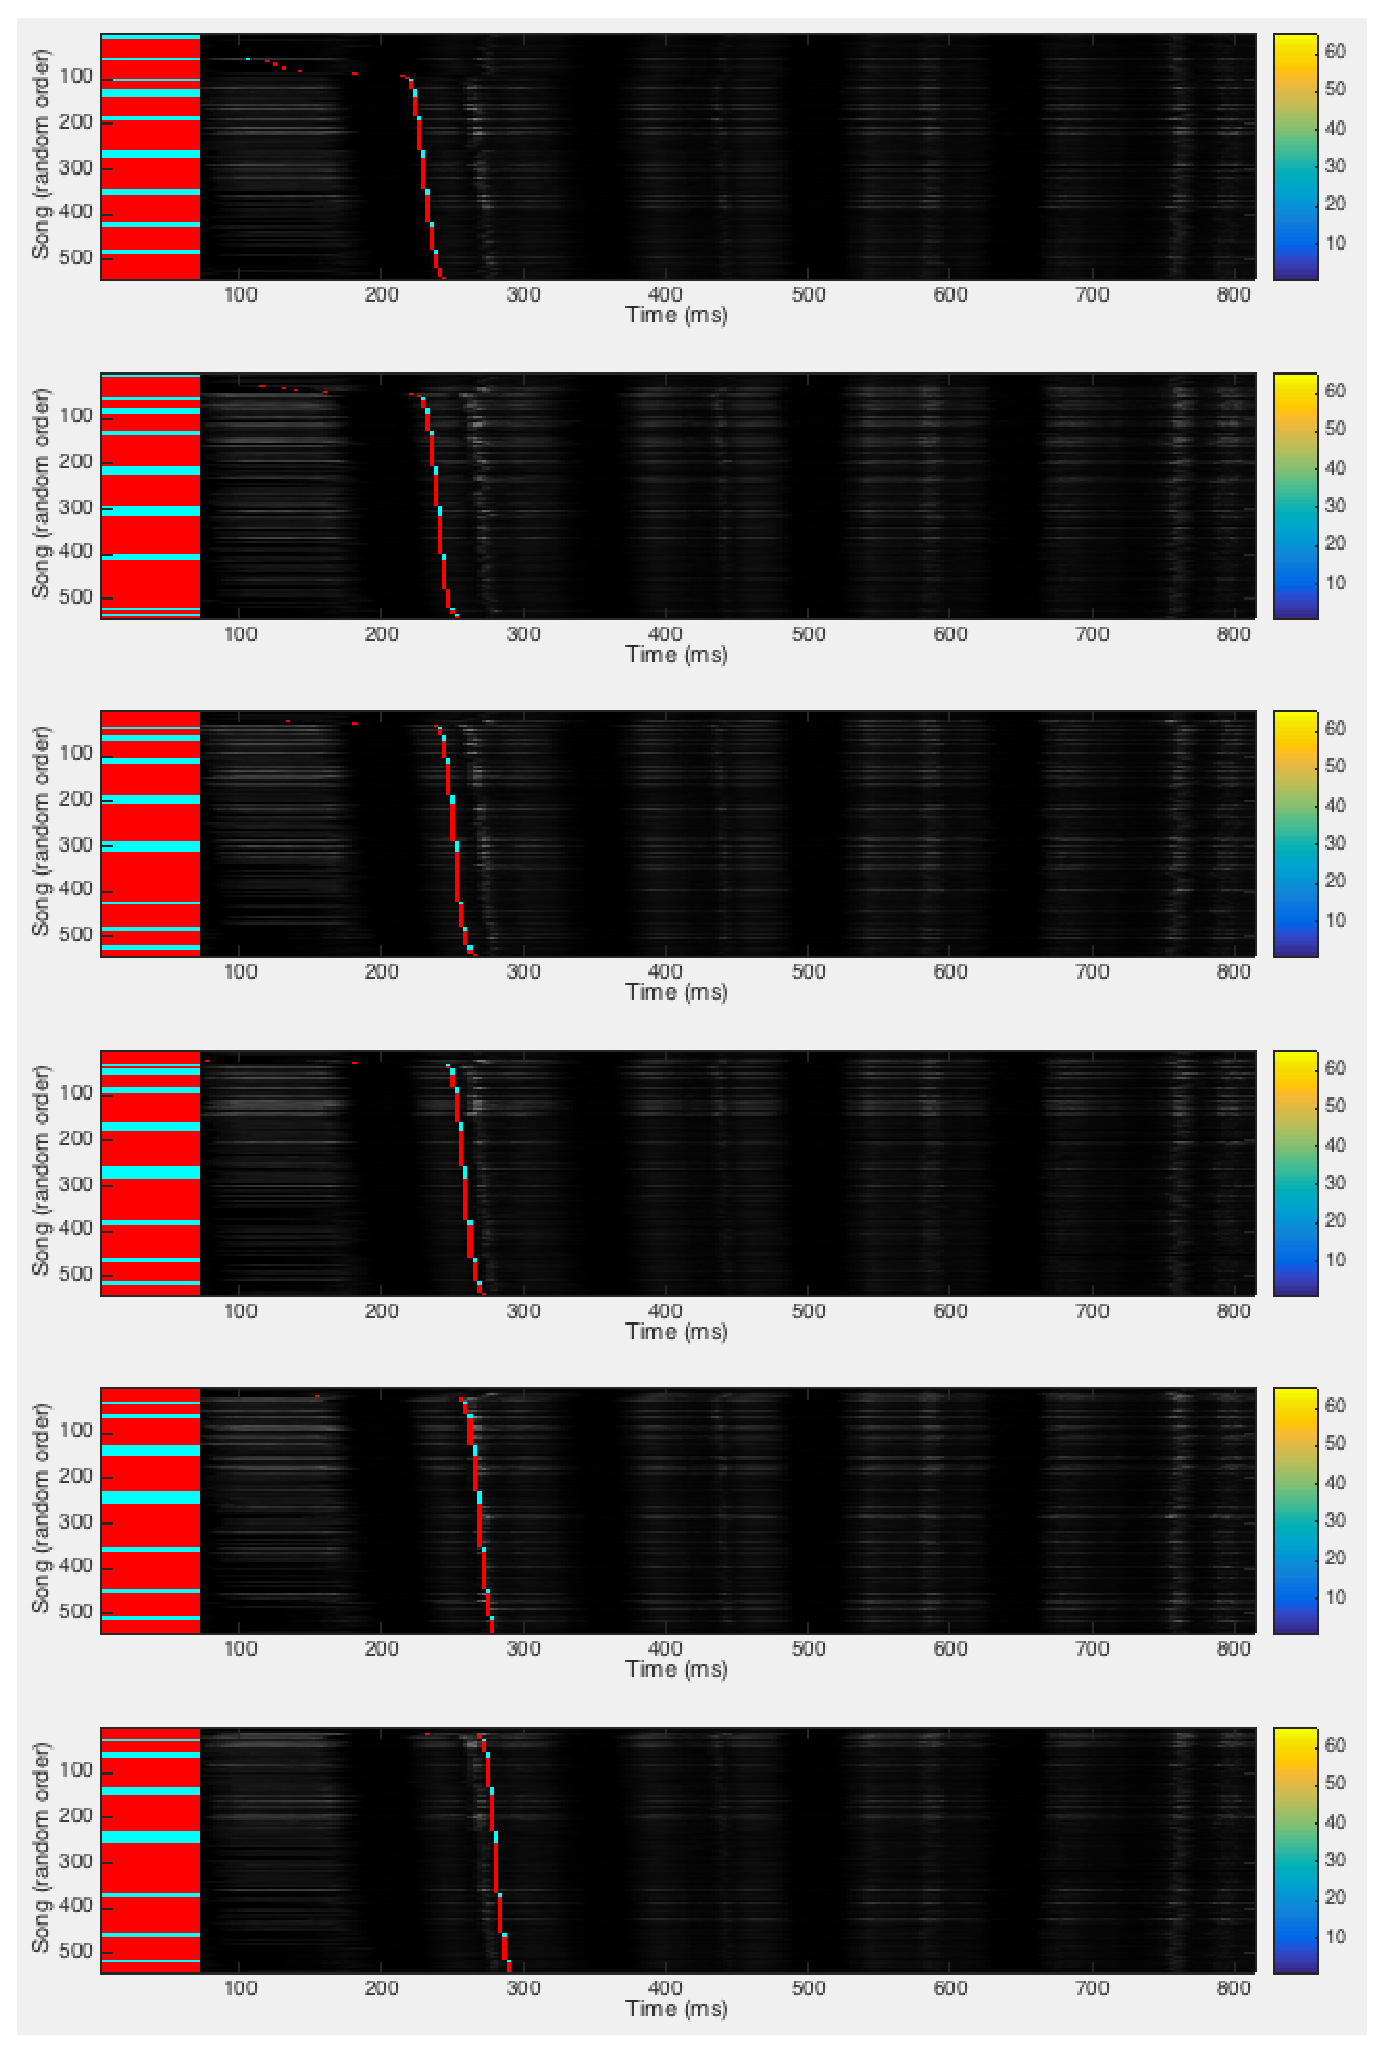
\includegraphics[width=\textwidth]{6_syllables_out}
    \caption{Detection results. Each plot shows detection events for
      the corresponding syllable as shown in
      \fig{fig:sixsyllables}. The horizontal axis is time, and the
      vertical axis is the index of the 526 single song
      presentations. The grey shading shows the total audio energy of
      song Y at time X. The bar on the left is the same width as the
      detection window, so no detection events can happen within that
      region, and its colour code shows training songs to the right of
      red regions and unseen test songs to the right of cyan
      regions. For visualisation of the distribution, songs have been
      stably sorted by the time of detection events.}
  \label{fig:sixsyllables_out}
\end{figure}

\begin{figure}
  \includegraphics[width=\textwidth]{6_syllables_roc}
  \caption{ROC curves for the detection of targets shown in Figure~\ref{fig:sixsyllables}. The first one, at the beginning of a syllable, is the most difficult to detect, and as more structure emerges in the current syllable, accuracy approaches 100\%.}
  \label{fig:roc}
\end{figure}

\begin{figure}
  \includegraphics[width=\textwidth]{timing}
  \caption{Timing curve for a syllable running a test file generated by training.}
  \label{fig:timing}
\end{figure}

\section{Case Study?}
\label{sec:case}

Jeff is using the detector for something cool, and it might be fun to get him to describe it in a paragraph or two.\marginpar{Do we want to include a case study? I think the paper is on the long side already, but it might be interesting and let Jeff earn that coauthorship ;)}

Failing that, I can immediately do song-aligned X spike rasters if lw95rhp is still willing to sing\dots but I have not heard him do so lately.

\section{Conclusion}
\label{sec:conclusion}

This syllable detector is appropriate for zebra finch song.  It offers
the following benefits:
\begin{itemize}
\item False positive and false negative rates can be well under 1\%.
\item Latency and jitter are both in the range of 2 milliseconds.
\item Works on a wide range of target syllables.
\item Requires minimal hand-tuning.
\item Runs in realtime on inexpensive consumer-grade hardware---we use the Mac Mini with 8GB RAM.
\item We recommend training the network on a computer with at least 32GB of RAM.
\end{itemize}
It has not been evaluated in other species, and the high accuracy presented here relies on zebra-finch--like consistency of song.

\appendix

\section{Resources}
\label{sec:resources}

\begin{description}
  \item[Song alignment:] Last we checked, Jeff Markowitz's song
    alignment software could be found at \\
    {\tt https://github.com/jmarkow}.

    \item[Training the neural network:] Our \marginpar{Fix the
      location! If going live, I should reorganise my repository, and
      also clean up the code.}  implementation of the syllable
      detector training code is available under the GNU GPL at:
      \\ {\tt https://github.com/bwpearre/}

    \item[Runtime:] The Swift implementation for executing the trained
      network:\\
      {\tt https://github.com/nathanntg/syllable-detector}
\end{description}

\bibliographystyle{plainnat}
\bibliography{rl}

\end{document}

